\documentclass{article}
\usepackage[a4paper, total={6.5in, 10in}]{geometry}
\setlength{\parindent}{0pt}
\usepackage{tcolorbox}
\tcbset{colback=white!94!black, colframe=black!60!white, coltitle = white, boxrule=0.8pt, arc=2mm}
\newtcolorbox{boxs}[2][]{title= #2,#1}
\usepackage{datetime2}
\usepackage[british]{babel}
\usepackage{amsfonts}
\usepackage{amsmath}
\usepackage{tikz}
\usepackage{tikz-3dplot}

\title{\textbf{Vectors}}
\author{Robert O'Connell}
\date{22nd September 2025}
\begin{document}
\maketitle
\vspace{5mm}

\section*{Vectors}
Vectors are geometric objects that have magnitude and direction \\
We will use $(x,y)$ to denote a point in $\mathbb{R}^2$ and $\langle x,y \rangle$ to denote a vector
in $\mathbb{R}^2$
\begin{itemize}
    \item Geometrically a vector is a directed line segment
    \item Algebraically it is determined by its coordinates
\end{itemize}
\subsection*{\(\mathbb{R}^n\)}
\begin{align*}
    \mathbb{R}^n &= \{\vec{v} = \langle v_1, v_2, \dots , v_n \rangle \mid v_1, v_2, \dots , v_n \in \mathbb{R},\, n \in \mathbb{N}\} \\
    &= \text{set of all ordered $n$-tuples of real numbers}
\end{align*}



\subsubsection*{Unit Vectors}
    A unit vector is a vector of length 1 for a given vector \(\vec{v} \in \mathbb{R}^n\). The direction of \(\vec{v}\)
    is \(\frac{1}{||\vec{v}||}\)

\subsubsection*{Basis Vectors}
\(\{ \langle 1,0 \rangle, \langle 0,1 \rangle \}\) are the standard basis vectors in \(\mathbb{R}^2\)
\\
\(\{ \langle 1,0,0 \rangle, \langle 0,1,0 \rangle, \langle 0,0,1 \rangle \}\) are the standard basis vectors in \(\mathbb{R}^3\)
\\
These are often denoted by \(\vec{i}, \vec{j}, \vec{k}\) respectively
\vspace{5mm}


\section*{Operations Defined on Vectors}
\subsection*{Magnitude of a vector.}
The magnitude of a vector $\vec{v} = \langle v_1, v_2, \dots , v_n \rangle \in \mathbb{R}^n$ is 
defined to be the distance from $(v_1, v_2, \dots , v_n)$ to the origin in $\mathbb{R}^n$
\[
\mid\mid\vec{v}\mid\mid = \mid\vec{v}\mid = \sqrt{{v_1}^2+{v_2}^2+\dots {v_n}^2}
\]

\subsection*{Addition of vectors}
Suppose $\vec{v}, \vec{w} \in \mathbb{R}^n$
\[
    \vec{v} = \langle v_1, v_2, \dots , v_n \rangle
\]
\[
    \vec{w} = \langle w_1, w_2, \dots , w_n \rangle
\]
We define $\vec{v} + \vec{w} = \langle v_1 + w_1, v_2 + w_2, ... , v_n + w_n \rangle$

\begin{itemize}
    \item Algebraically we add components
    \item Geometrically $\vec{v} + \vec{w}$ is the directed line segment that is a diagonal of the
    parallelogram formed by $\vec{v}$ and $\vec{w}$
\begin{center}
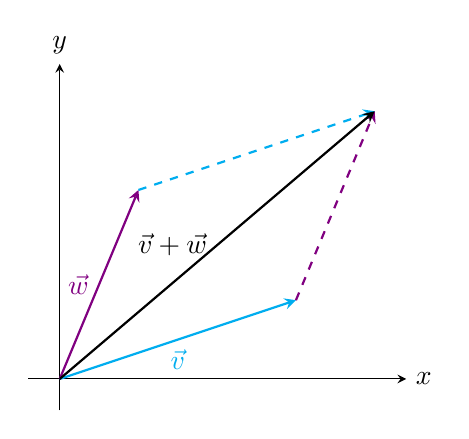
\begin{tikzpicture}[scale=2,>=stealth]

% Axes
\draw[->] (-0.2,0) -- (2.2,0) node[right]{$x$};
\draw[->] (0,-0.2) -- (0,2) node[above]{$y$};

% Vectors u and v
\draw[->,thick,cyan] (0,0) -- (1.5,0.5) node[midway,below]{$\vec{v}$};
\draw[->,thick,violet] (0,0) -- (0.5,1.2) node[midway,left]{$\vec{w}$};

% Translate v to tip of u
\draw[->,thick,violet,dashed] (1.5,0.5) -- (2,1.7);

% Translate u to tip of v
\draw[->,thick,cyan,dashed] (0.5,1.2) -- (2,1.7);

% Resultant vector
\draw[->,thick,black] (0,0) -- (2,1.7) node[midway,left]{$\vec{v}+\vec{w}$};

\end{tikzpicture}
\end{center}
\end{itemize}

\subsection*{Scalar multiplication of vectors}
A scalar is a real number, $\lambda \in \mathbb{R}$
\\
Let $\lambda \in \mathbb{R}, \vec{v} \in \mathbb{R}^n$,
\\
$\lambda\vec{v}$ is defined to be
\[
    \langle \lambda v_1, \lambda v_2, \dots , \lambda v_n \rangle
\]
\begin{itemize}
\item Geometrically $\lambda\vec{v}$ points in the same direction as $\vec{v}$ if $\lambda > 0 $ and
in the opposite direction if \(\lambda < 0\) and \(\lambda\vec{v}\) has magnitude \(\mid\lambda\mid\mid\vec{v}\mid\)
\end{itemize}

\subsection*{Dot Product (Scalar Product)}
Let \(\vec{v}, \vec{w} \in \mathbb{R}^n\)
\[
    \vec{v} = \langle v_1, v_2, \dots , v_n \rangle
\]
\[
    \vec{w} = \langle w_1, w_2, \dots , w_n \rangle
\]
The dot product of \(\vec{v}\) and \(\vec{w}\) is denoted by \(\vec{v}\cdot\vec{w}\)
and is defined as follows
\[
\vec{v}\cdot\vec{w} = v_1w_1 + v_2+w_2+\dots +v_nw_n \quad \in \mathbb{R}
\]
Geometrically the dot product can be defined as
\[
\vec{v} \cdot \vec{w} = \mid\mid\vec{v}\mid\mid \mid\mid\vec{w}\mid\mid \cos \theta
\]
where \(\theta\) is the angle \((\leq\pi)\) between the two vectors
\subsubsection*{Orthogonality}
Two vectors \(\vec{v}, \vec{w} \in \mathbb{R}^n\) are said to be orthogonal if and only if
\(\vec{v} \cdot \vec{w} = 0\), i.e. the angle between the two vectors if \(\frac{\pi}{2}\)
% insert note on how the dot product shows the degree to which two unit vectors point in the same direction

\subsection*{Cross Product (Vector Product)}
Note that the cross product is only defined in \(\mathbb{R}^3\)




\section*{Properties of the operations}
Let \(\vec{v},\vec{w},\vec{q} \in \mathbb{R}^n, \quad \lambda \in \mathbb{R}\)
\begin{enumerate}
\item \(\vec{v}\cdot\vec{w} = \vec{w}\cdot\vec{v} \)
\item \(\lambda(\vec{v}+\vec{w}) = \lambda\vec{v} + \lambda\vec{w}\)
\item \(\lambda(\vec{v}\cdot\vec{w}) = (\lambda\vec{v})\cdot\vec{w} = \vec{v}\cdot(\lambda\vec{w})\)
\item \(\vec{v}\cdot\vec{v} = \mid\mid\vec{v}\mid\mid^2\)
\item \(\vec{v}\cdot\vec{w} = \mid\mid\vec{v}\mid\mid\mid\mid\vec{w}\mid\mid\cos\theta\)
\item \(\vec{v}\cdot(\vec{w} + \vec{q}) = \vec{v}\cdot\vec{w} + \vec{v}\cdot\vec{q}\)
\end{enumerate}
\vspace{5mm}
\textbf{Proofs of the Properties}
\begin{enumerate}
\item \begin{align*}
    \vec{v}\cdot\vec{w} &= v_1w_1+v_2w_2+\dots+v_nw_n \\
    &= w_1v_1 + w_2v_2+\dots w_nv_n \quad \text{(Commutivity of multiplication of real numbers)} \\
    &= \vec{w}\cdot\vec{v}
\end{align*}
\item 
\begin{align*}    
    \lambda(\vec{v}+\vec{w}) &= \lambda(v_1+w_1+v_2+w_2+\dots+v_n+w_n) \\
    &= \lambda(\vec{v_1}+ \vec{v_2}+\dots + \vec{v_n}) + \lambda(\vec{w_1}+ \vec{w_2}+\dots + \vec{w_n}) \quad \text{(Distributive law of real numbers)}\\
    &= \lambda\vec{v} + \lambda\vec{w} \\
\end{align*}
\item \begin{align*}
    \lambda(\vec{v}\cdot\vec{w}) &= \lambda(v_1w_1+v_2w_2+\dots+v_nw_n) \\
    &= \lambda(v_1w_1) + \lambda(v_2w_2) + \dots + \lambda(v_nw_n) \quad \text{(Distributive law of real numbers)} \\
    &= v_1(\lambda w_1) + v_2(\lambda w_2) + \dots + v_n(\lambda w_n) \\
    &= \vec{v}\cdot(\lambda\vec{w})
\end{align*}
\item \begin{align*}
    \vec{v} \cdot \vec{v} &= (v_1)^2 + (v_2)^2 + \dots + (v_n)^2 \\
    &= (\sqrt{(v_1)^2 + (v_2)^2 + \dots + (v_n)^2})^2 \\
    &= (\mid\mid \vec{v} \mid\mid)^2
\end{align*}
\item to be completed
\end{enumerate}

\end{document}